

\chapter{Desenvolvimento}


\subsection{Montagem da parte elétrica}

Os componentes foram ligados usando cabos do tipo jumper e protoboard para encaixar o microcontrolador e os drivers,
essa ligação foi útil para realizar os testes, porém o uso cabos do tipo jumper e protoboard podem oferecer mau contado, causando falhas no funcionamento do robô.
Para realizar testes finais, realizar junção dos cabos, e soldar os cabos a conectores JST devem resolver o problema de mau contado.


\subsubsection{Ligação dos componentes}
Cada motor precisa de 2 sinais de PWM, então foi necessário usar 6 pinos de PWM do STM32, as duplas de pinos que suportam PWM foram $P_{B6}$ - $P_{B7}$, $P_{B8}$ - $P_{B9}$ e $P_{A9}$ - $P_{A10}$, respectivamente para os motores 1, 2 e 3
E para cada encorder de motor, foi necessário mais 6 pinos, 2 pinos para cada fase dos 3 encoders, $P_{B0}$ - $P_{B1}$, $P_{A6}$ - $P_{B7}$ e $P_{B10}$ - $P_{B11}$, também respectivamente para os motores 1, 2 e 3, sendo os  $P_{B1}$, $P_{B7}$ e $P_{B11}$ definidos para a Fase A do encoder
A alimentação dos encoders será feito pelo pino de 3.3v do STM32, e o GND também vindo do microcontrolador.
O Módulo bluetooth HC-05 terá alimentação sendo fornecida pelo pino de 5v do microtrolador (GND sendo o mesmo usado para os encoders).
Já a comunicação serial será feita conectando o TXD do módulo com o pino $P_{A3}$, que é o pino RX2 (RX da $USART\_2$), e o RXD do módulo conectado ao $P_{A2}$, pino TX2 (TX da $USART\_2$).
Embora o HC-05 trabalhe com UART, o protocolo USART é compatível com UART, podendo usar os pinos de uma USART como se fossem uma UART.

Os pinos de PWM são conectados nos drivers DVR8833, com  $P_{B6}$, $P_{B8}$ e $P_{A9}$ como inputs nos pinos $IN1$ de cada driver, e os demais pinos conectados aos pinos $IN2$.
A alimentação dos drivers é feita por uma fonte de 6v, e os pinos $OUT1$ e $OUT2$ dos drivers conectados respectivamente as entradas $M1$ e $M2$ dos motores. A figura \ref{fig:diagrama_montagem} contém o diagrama com as ligações descritas.

\begin{figure}[htb]
	\centering
	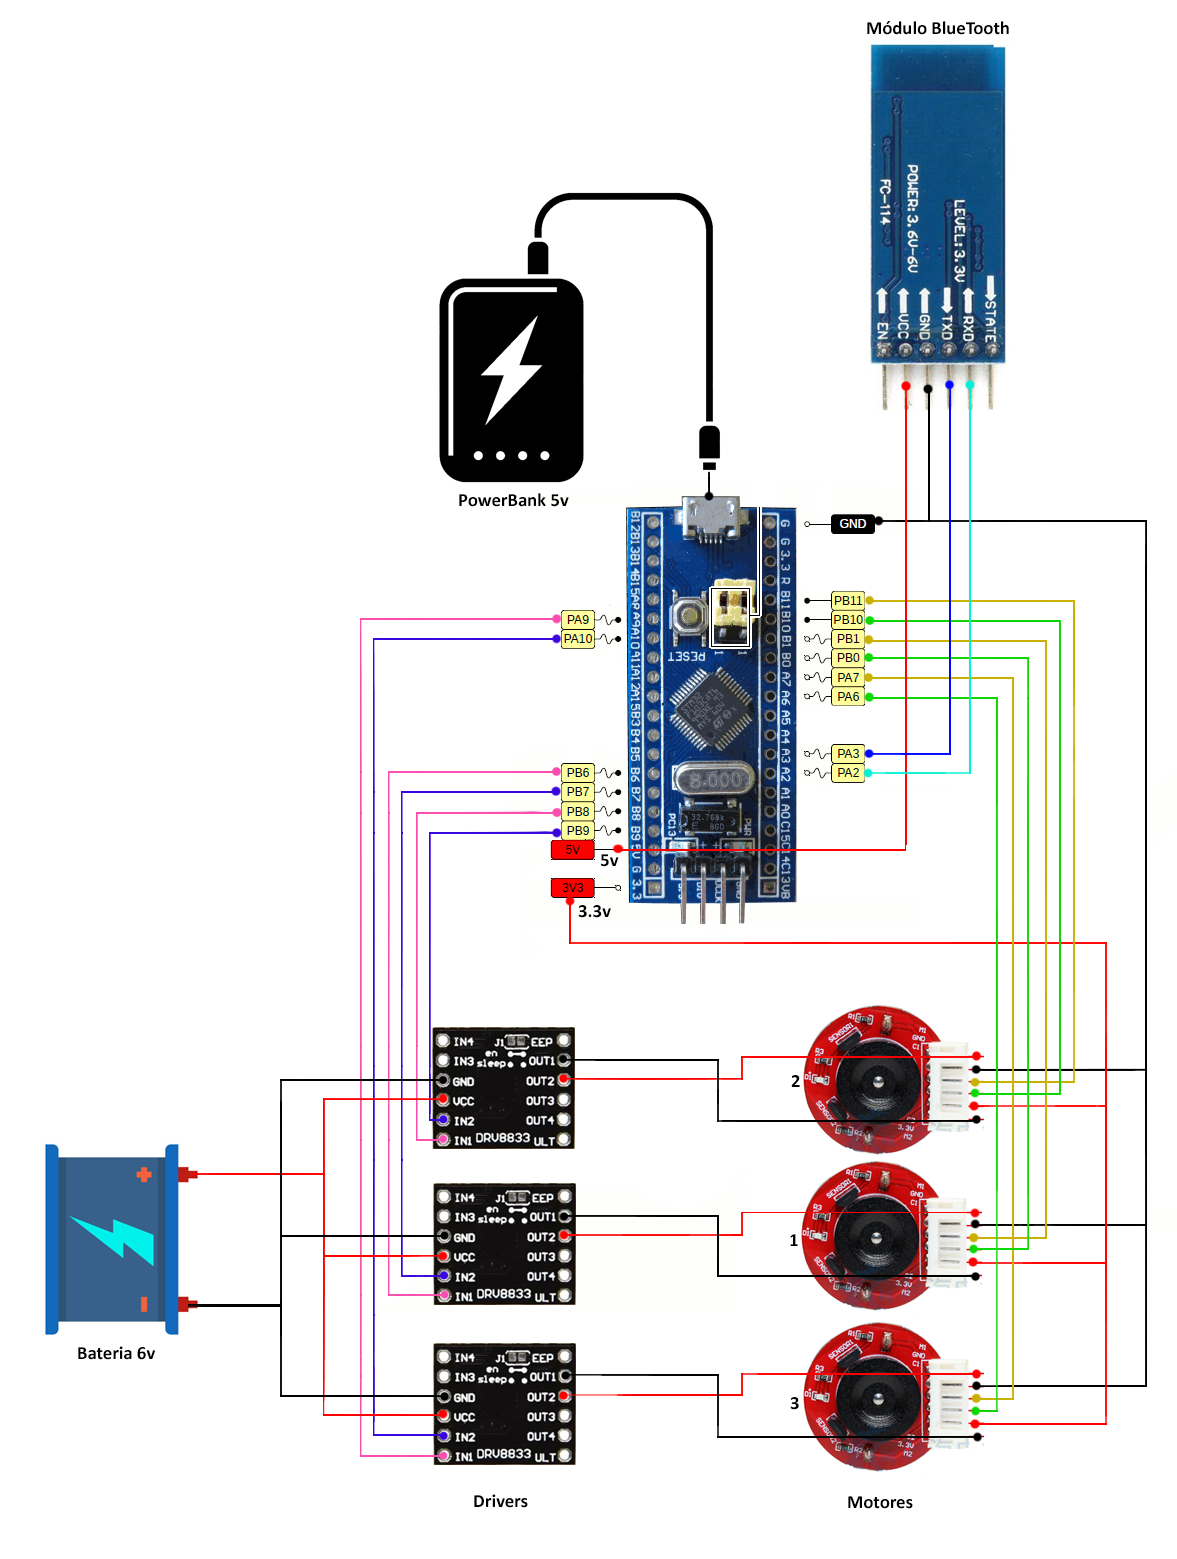
\includegraphics[width=1.0\textwidth]{figures/diagrama_montagem}
	\caption{Diagrama de montagem dos componentes}
	\label{fig:diagrama_montagem}
\end{figure}


\subsubsection{Modelagem e fabricação da estrutura}

O desenvolvimento das peças usadas na estrutura do robô foram feitas usando AutoCAD, o chassi principal que possui a geometria circular do robô foi desenhado com base nas medidas finais do robô,
com foco no raio até o centro das rodas, o raio planejado é de 100mm. Os mancais foram planejados com base nas dimensões dos motores. 

As figuras relacionadas ao CAD, podem ser encontradas no anexo \ref{att_fabricao_montagem_cad}, quanto a modelagem,
anexo \ref{att_fabricao_montagem_modelagem}, e impressão 3D e montagem, anexo \ref{att_fabricao_montagem_impressao}.



\subsection{Controle de velocidade}

\subsubsection{Medição de velicidade do motor}

Como encoder possuí dois sinais de onda quadadra defasadas em 90º, fase A e fase B, cujos vales e picos são valores lógicos HIGH e LOW, 
e direção de rotação do motor pode ser definida pela diferença entre as fases, se fase A esta adiantada ou atrasada em relação a fase B
É possível calcular a velocidade com base nas subidas da onda quadrada de uma fase, e o valor logico da outra fase no momento da subida.
Por exemplo,  observando a fase B, toda vez em que há uma subida, se o valor da fase A for alto, então incrementar +1 em um contador, se a fase A tiver valor baixo, então incrementar -1 no contador.
Quando o valor da fase A for alto, então o motor esta rodando em um sentido,  quando o valor  for baixo, então o motor esta rodando no sentido contrário.
Medindo o valor do contador por um $\Delta_{T}$, se resulta na quantidade de pulsos por segundo.
Para converter de pulsos por segundo para RPM, basta dividir pela resolução do motor+encoder,  que é de 1:34 do motor, e 11 pulsos por rotação do encoder, o que resulta em 374,
e multiplicar por 60 para ter o resultado em rotações por minuto.

\begin{tikzpicture}[node distance=2cm]

    \node (start) [startstop] {início loop};
    \node (pro1) [process, below of=start] {ENQUANTO DELTA T};
    
    \node (in1) [io, right of=pro1, xshift= 4cm] {QUANDO FASE B = SUBIDA};
    
    \node (dec1) [decision, below of=in1, yshift=-2cm] {SE FASE A = 1};
    \node (pro1a) [process, below of=dec1, yshift= -2cm] {INCREMENTAR CONTADOR em +1};
    \node (pro1b) [process, right of=dec1, xshift= 3cm] {INCREMENTAR CONTADOR em -1};
    
    
    \node (count) [process, below of=pro1, yshift= -9cm] {CONTADOR DIVIDO POR DELTA T};
    
    \draw [arrow] (start) -- (pro1);
    \draw [arrow] (pro1) -- node[anchor=north] {sim} (in1);
    \draw [arrow] (in1) -- (dec1);
    \draw [arrow] (dec1) -- node[anchor=east] {sim} (pro1a);
    \draw [arrow] (dec1) -- node[anchor=north] {não} (pro1b);
    
    \draw [arrow] (pro1) -- node[anchor=east] {não} (count);

\end{tikzpicture}



Na implementação dessa lógica no STM32, o desafio foi a definição do $\Delta_{T}$,
Se o $\Delta_{T}$ for muito pequeno, o resultados de pulsos por segundo pode tender ao infinito, gerando valores muito altos.
Na figura \ref{fig:medidas_altas} em laranja, esta o resultado do rpm considerando o $\Delta_{T}$ como o tempo entre os ciclos do micrcontrolador.
A outra opção, foi definir um $\Delta_{T}$ fixo, definindo uma frequencia de medição pré definida, e o resultado pode ser visto em azul na figura \ref{fig:medidas_altas}
Essa outra opção de $\Delta_{T}$ resultou em um sinal que tem uma componente em alta frequência com uma amplitude até consideral.
Analisando os dois sinais no dominio da frequêcia na figura \ref{fig:frequencia_medidas_altas}, o espectro em frequência do sinal em laranja possui amplitudes muitos semelhante em todo espectro, mas o espectro do sinal em azul, fica bem claro que em altas frequencias é composto mais por ruidos
e as frequencia médias tem amplitude menor em relação as frequências baixas, o que torna mais fácil aplicar um filtro passa-baixa para reduzir as frenquências médias e altas.

A figura \ref{fig:passa_baixa_teste}, mostra um dos teste de filtro passa baixa, em o sinal em laranja ainda persiste esses valores tentendo ao infinito, devido a ampliture eles se tornam um pouco dificil de serem retirados.
Mas o sinal em azul acaba tendo um resultado melhor depois do filtro, muito semelhando ao sinal em laranja.
Com base nesse resultado, foi decidido seguir com o método em que o $\Delta_{T}$ é definido por uma frequência pré definida.


\begin{figure}[h]
    \centering
    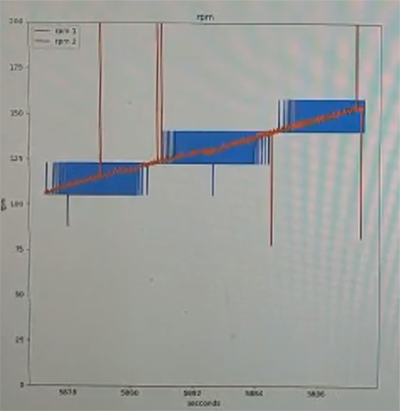
\includegraphics{figures/medidas_altas}
    \caption{Problemas com delta T muito pequeno}
    \label{fig:medidas_altas}
\end{figure}

\begin{figure}[h]
    \centering
    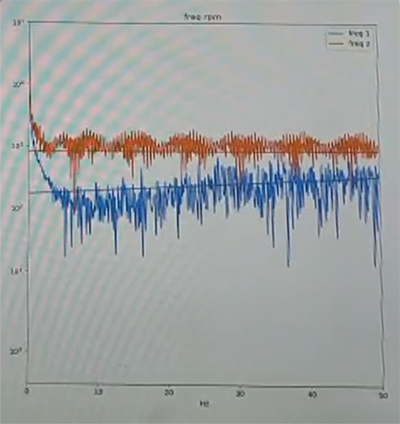
\includegraphics{figures/frequencia_medidas_altas}
    \caption{Frequências}
    \label{fig:frequencia_medidas_altas}
\end{figure}

\begin{figure}[h]
    \centering
    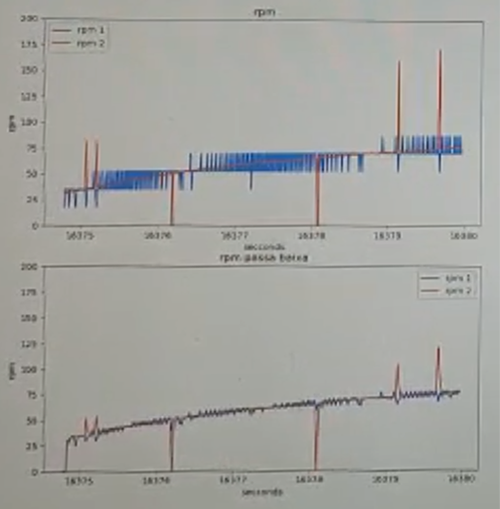
\includegraphics{figures/passa_baixa_teste}
    \caption{Passa baixa teste}
    \label{fig:passa_baixa_teste}
\end{figure}


Com o método definido, foi definido um $\Delta_{T}$ em 100hz eu um filtro passa baixa em 2hz
As imagens no anexo \ref{att_medicao_motores}, mostra as imagens comparando o sinal original e o sinal filtrado para cada motor.
A equação \ref{eqn:equacao_diferenca} a seguir é a equação de diferença do filtro, considerando uma amostragem de 100hz e frequência de corte em 2hz.

\begin{equation}
    \begin{split}
        y[k] = 0.0591174 \cdot u \left[ k \right] +  0.0591174 \cdot u[k - 1] + 0.88176521 \cdot y[k - 1]
    \end{split}
    \label{eqn:equacao_diferenca}
\end{equation}

\subsubsection{Curva PWM x RPM - problema da não linearidade}

Depois de definido como calcular a velocidade o próximo desafio foi lidar com a não linearidade entre o PWM e o resultado medido em RPM.
Como pode ser visto na figura \ref{fig:grafico_pwm_x_rpm}, na comparação entre o valor do PWM e o RPM no tempo.

\begin{figure}[htb]
	\centering
	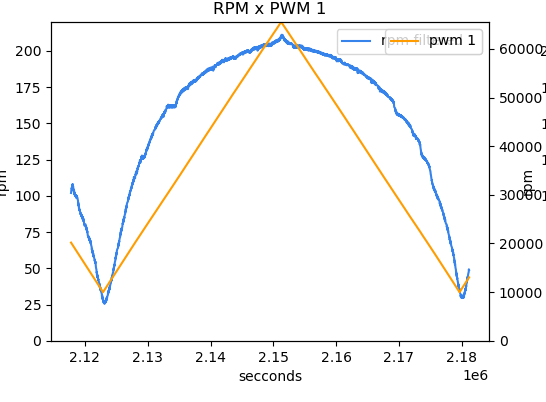
\includegraphics{figures/pwm_x_rpm}
	\caption{Curva PWM e RPM no tempo}
	\label{fig:grafico_pwm_x_rpm}
\end{figure}

Considerando essa não linearidade, foram realizadas 15k medições em PWM vs RPM para definir uma equação que pudesse relacionar o PWM com o RPM.
Como pode ser observado na figura  \ref{fig:medicao_pwm_x_rpm_dados_brutos}, os resultados possuem uma tendência, mas possuem alguns pontos fora da curta.
devido ao esses ruídos nas medições ss dados foram tratatos para obter valores médios dos resultados usando python,
o código pode ser visto no anexo \ref{att_limpeza_python}.

\begin{figure}[htb]
	\centering
	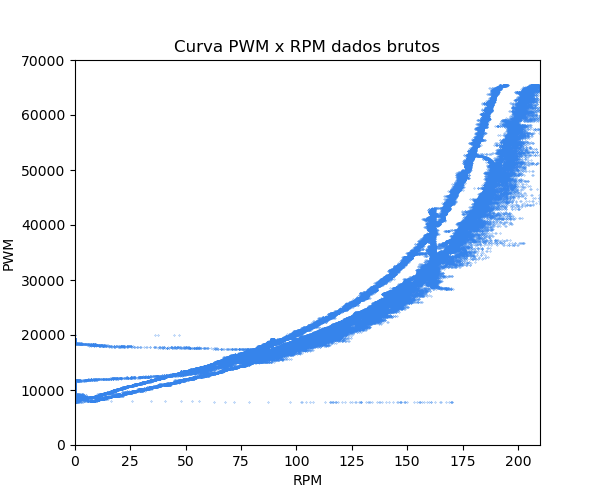
\includegraphics{figures/curva_pwm_x_rpm_dados_brutos}
	\caption{Curva PWM x RPM dados brutos}
	\label{fig:medicao_pwm_x_rpm_dados_brutos}
\end{figure}


O resultado da limpeza dos dados pode ser vizualizado na figura \ref{fig:medicao_pwm_x_rpm_dados_medios}.
Após a limpeza dos dados, os dados foram importados para o matlab, anexo \ref{att_matlab},
para obter um polinômio que possa definir a curva, o polinômio resultante é a equação \ref{eqn:polimonio_rpm}, e a figura \ref{fig:curva_ajustada} representa a curva ajustada.
A equação do polinômio foi inserida no código do micrcontrolador, foi testado definir um RPM de 150, e a tabela \ref{medicao_motores} trás uma amostra dos resultados dos RPMs de cada motor.
Com essa equação é mais fácil definir um comportamento linear, facilitando a aplicação de um controle PDI.

\begin{equation}
    \begin{split}
        0.0001131x^{4} + -0.03064x^{3} + 2.993x^{2} + -1.257x + 9017
    \end{split}
    \label{eqn:polimonio_rpm}
\end{equation}

\begin{figure}[htb]
	\centering
	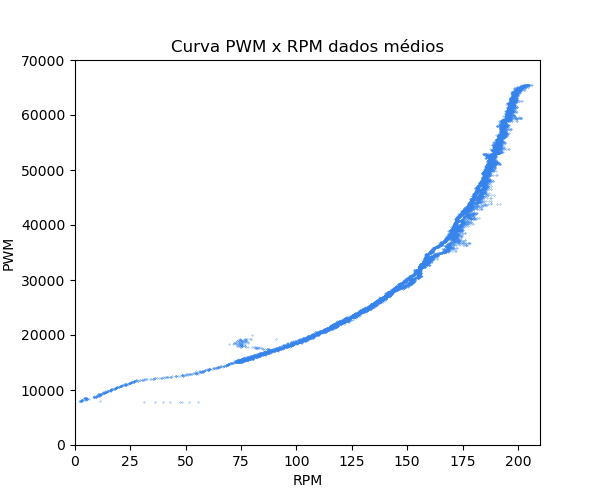
\includegraphics{figures/curva_pwm_x_rpm_dados_medios}
	\caption{Curva PWM x RPM dados médios}
	\label{fig:medicao_pwm_x_rpm_dados_medios}
\end{figure}

\begin{figure}[htb]
	\centering
	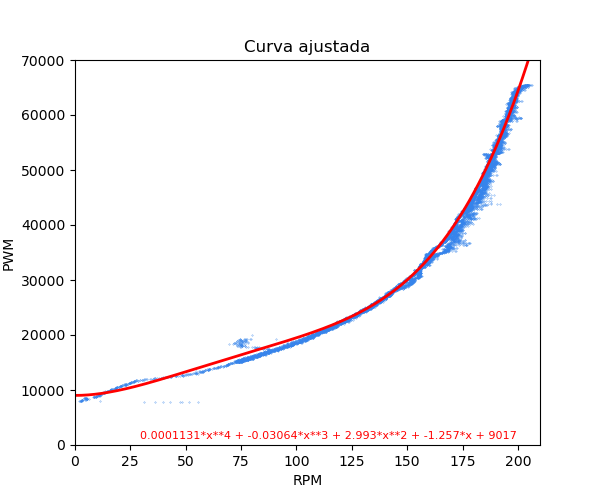
\includegraphics{figures/curva_ajustada}
	\caption{Curva ajustada}
	\label{fig:curva_ajustada}
\end{figure}



\begin{quadro}[htb]
	\caption{\label{medicao_motores}Medição rpms motores}
	 \begin{tabular}{|c|c|c|c|c|}
		\hline
		\textbf{$Tempo_{seg}$} & \textbf{$RPM_{definido}$} & \textbf{$RPM_{real_{1}}$} & \textbf{$RPM_{real_{2}}$} & \textbf{$RPM_{real_{3}}$} \\ \hline
		52.954 & 150.00  & 141.03 & 162.69 & 149.82 \\ \hline
		52.954 & 150.00  & 141.43 & 162.43 & 149.18 \\ \hline
		53.000 & 150.00  & 140.83 & 162.19 & 148.61 \\ \hline
		53.000 & 150.00  & 140.30 & 161.98 & 149.06 \\ \hline
		53.000 & 150.00  & 140.79 & 161.80 & 149.46 \\ \hline
		53.000 & 150.00  & 141.21 & 161.64 & 148.86 \\ \hline
		53.046 & 150.00  & 141.59 & 161.49 & 149.28 \\ \hline
		53.046 & 150.00  & 141.92 & 161.37 & 149.65 \\ \hline
		53.046 & 150.00  & 141.26 & 161.25 & 149.02 \\ \hline
		53.046 & 150.00  & 140.68 & 162.11 & 148.48 \\ \hline
		53.046 & 150.00  & 141.12 & 162.86 & 148.94 \\ \hline
		53.092 & 150.00  & 141.51 & 162.57 & 149.35 \\ \hline
		53.092 & 150.00  & 141.85 & 162.32 & 148.76 \\ \hline
		53.092 & 150.00  & 141.20 & 162.09 & 149.19 \\ \hline
		53.092 & 150.00  & 140.63 & 161.90 & 149.57 \\ \hline
	\end{tabular}
\end{quadro}


\subsection{Aplicativo andriod - Envio de dados via bluetooth}



\subsection{Implementação da medição de rpm e filtro passa baixa no microcontrolador}